\documentclass[border=2mm]{standalone}
\usepackage{amsmath}
\usepackage{tikz}
\usetikzlibrary{arrows.meta, decorations.pathreplacing}

\usepackage{xcolor}
\definecolor{den-1}{HTML}{111111}   % Đen #111111
\definecolor{den-2}{HTML}{222222}   % Đen #222222
\definecolor{den-3}{HTML}{333333}   % Đen #333333
\definecolor{den-4}{HTML}{444444}   % Đen #444444
\definecolor{den-5}{HTML}{555555}   % Đen #555555
\definecolor{den-6}{HTML}{666666}   % Đen #666666

\definecolor{do-1}{HTML}{440000}   % Đỏ #440000 trầm hơn, hợp với đen #111111
\definecolor{do-2}{HTML}{660000}   % Đỏ #660000 sẫm, hợp với đen #222222
\definecolor{do-3}{HTML}{880000}   % Đỏ #880000 đậm vừa, hợp với đen #333333
\definecolor{do-4}{HTML}{AA0000}   % Đỏ #AA0000 tươi vừa, hợp với đen #444444
\definecolor{do-5}{HTML}{CC0000}   % Đỏ #CC0000 tươi hơn, hợp với đen #555555
\definecolor{do-6}{HTML}{EE0000}   % Đỏ #EE0000 sáng hơn, hợp với đen #666666

\tikzset{
  vat/.style = {->, line width=3pt, color=main-dark},
  anh/.style = {->, line width=3pt, color=main-dark!50},
  tia/.style = {line width=1.5pt, color=secondary-dark, opacity=.5},
  truc/.style = {<->, dotted, line width=1.5pt, color=secondary-dark},
  diem/.style = {filldraw, color=main-dark, circle, radius=0.05}
}


\begin{document}
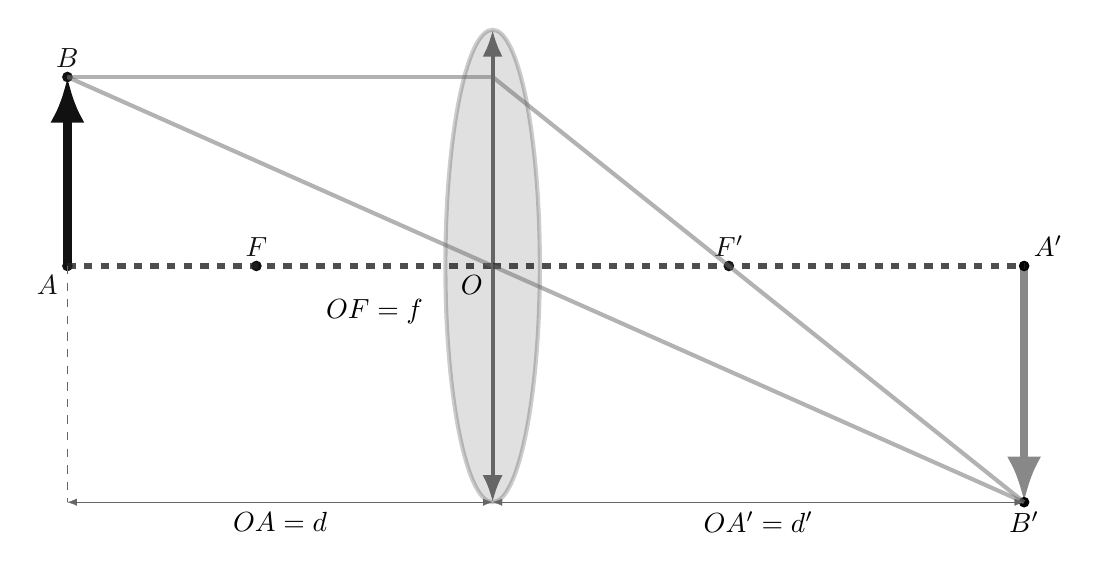
\begin{tikzpicture}[scale=1.2, >=Latex]

  % Các thông số
  \def\f{2.5}      % tiêu cự f
  \def\d{4.5}      % khoảng cách vật đến thấu kính
  \def\h{2}        % chiều cao vật
  \def\O{0}        % vị trí quang tâm O

  % Tính khoảng cách ảnh d'
  \pgfmathsetmacro{\dpval}{(\d*\f)/(\d - \f)}
  \pgfmathsetmacro{\hpval}{-\h * \dpval / \d} % chiều cao ảnh thật (âm)

  % Trục chính
  % \draw[->] (-1.5*\d, 0) -- (\dpval + 2, 0) node[below right] {Trục chính};

  % Thấu kính hội tụ (hình elip)
  \draw[line width=1.5pt, fill=den-6, opacity=0.2] (\O,0) ellipse (0.5 and 2.5);

  \draw[<->, line width=1.5pt, color=den-6!] (\O,-2.5) -- (\O,2.5);

  \node[below left] at (\O,0) {$O$};

  % Vật AB
  \draw[->, color=den-1, line width=3pt] (-\d,0) -- (-\d,\h);
  \filldraw[color=den-1] (-\d,0) circle (0.05) node[below left] {$A$};
  \filldraw[color=den-1] (-\d,\h) circle (0.05) node[above] {$B$};

  % Ảnh A'B'
  \draw[->, color=den-1!50, line width=3pt] (\dpval,0) -- (\dpval,\hpval);
  \filldraw (\dpval,0) circle (0.05) node[above right] {$A^\prime$};
  \filldraw (\dpval,\hpval) circle (0.05) node[below] {$B^\prime$};

  % Các tiêu điểm F và F'
  \filldraw[color=den-1] (\f, 0) circle (.05) node[above] {$F^\prime$};
  \filldraw[color=den-1] (-\f, 0) circle (.05) node[above] {$F$};

  % Nhãn khoảng cách OA = d và OA' = d'
  \draw[dashed, line width=2pt, color=den-2, opacity=.8] (-\d,0) -- (\O,0);
  \draw[dashed, line width=.1pt, color=den-6] (-\d,0) -- (-\d,-2.5);
  \draw[<->, line width=.1pt, color=den-6] (-\d,-2.5) -- (\O,-2.5);
  \node[below] at ({-\d/2}, -2.5) {$OA = d$};

  \draw[dashed, line width=2pt, color=den-2, opacity=.8] (\O,0) -- (\dpval,0);
  \draw[<->, line width=.1pt, color=den-6] (\O,-2.5) -- (\dpval,-2.5);
  \node[below] at ({(\O + \dpval)/2}, -2.5) {{$OA^\prime = d^\prime$}};

  \node[below] at ({-\f/2}, -.25) {$OF = f$};

  % Tia sáng: từ B song song trục chính, khúc xạ qua F
  \draw[line width=1.5pt, color=den-6, opacity=.5] (-\d,\h) -- (\O,\h); % tia tới
  \draw[line width=1.5pt, color=den-6, opacity=.5] (\O,\h) -- (\dpval,\hpval); % tia khúc xạ qua F

  % Tia sáng: từ B đi qua O
  \draw[line width=1.5pt, color=den-6, opacity=.5] (-\d,\h) -- (\dpval,\hpval);

\end{tikzpicture}
\end{document}
